\chapter{Conclusions and future work}
This chapter will bring together the results of this thesis, providing final thoughts on the theoretical and experimental work performed. The future of hydrogen separation membranes and their use in the hydrogen economy will be discussed. Finally future applciations and further improvements for the HIED will be described.

\section{Membranes for hydrogen separation}
\subsection{DFT for screening impurity resistant alloys}\label{simconc}
This thesis presented a methodology for fast screening of palladium alloy membrane compositions for resistence of impurities. The simulations involving sulphur samples were relatively accurate, and were able to successfully predict which membranes would perform the best when tested in chapter 5. The model however broke down for other impurities and this is due to the fact that the chosen simulation method is not accurate for weak interactions. \cite{dftbook1} Further development of the models should be performed in order to accurately predict the impact of these impurities. The model can also be expanded to predict the solubility of hydrogen within the palladium alloy membranes by combining monte carlo simulation techniques with cluster expansion simulations as has been performed by Scholl et al. \cite{SHOLL2007462} Future work could take combine these simulation methods to predict everything from the impurity interactions, to permeability and performance of the membranes. If such a system was developed it could greatly reduce the time taken to discover new alloy compositions. 

There is also scope for testing more membrane compositions. This thesis tested a limited number of alloy composition due to lack of computing power and time available. With HPC networks becoming more and more available \cite{morgan_burt_feldman_2020} a great number of alloys can be simulated quickly, allowing bespoke membrane compositions to be potentially found for any application. 

\subsection{Use for dense metal membranes in the hydrogen economy}
In this work we presented a use case for dense metal membranes as a material to perform hydrogen impurity enrichment to measure ISO 14687-2 impurities. As the hydrogen economy grows there will be other potential uses for such technology. 

There are already examples of industry capturing waste hydrogen from their processes and using it as a power source either through a fuel cell, or other means.\cite{doi:10.1177/0144598719839767} It is estimated that there are 100,000MW of waste hydrogen produced each year and therefore could result in a meaningful resource. \cite{cox} As more processes turn to this there is potential for a highly personalised market for dense metal membranes. Dense metal membranes provide ultrapure hydrogen suitable for use in fuel cells, therefore protecting the investment in any new type of energy utilization technology and this will become especially true as the cost of such membranes decreases through the development of stable ceramic supported membranes.

If combined with the simulation research discussed in section \ref{simconc} there could be potential for an highly linked membrane ecosystem. Where a plant owner can define the requirements for their hydrogen separation process, the optimal membrane can be found by a computational research provider, and finally manufactured into a module. This process is visualised in figure \ref{manuproc}. While palladium membranes will likely not replace PSA in the SMR process, due to the high levels of impurities found in these processes, however may be suitable for processes where hydrogen is often a byproduct such as ammonia, or certain pharmaceutical processes. 

\begin{figure}
    \centering
    
\includegraphics[width=\linewidth, keepaspectratio]{/Users/marc/Thesis/Chapter6/manuproc.png}
    \caption{Theoretical manufacturing process for a bespoke dense metal membrane with optimal composition calculated by a research provider, manufactured to specification, and delivered to the customer}
    \label{manuproc}
\end{figure}

Another potential use for dense metal membranes is in a potential hydrogen grid system. Projects such as HyGrid \cite{hygrid} aim to use the existing natural gas network in Europe as a storage medium for the hydrogenm economy, mixing hydrogen with natural gas to improve it's energy density and reduce the carbon footprint of the natural gas network. In addition to this there are several companies now offering hydrogen CHP systems for use in homes, which are powered using a fuel cell, to provide thermal energy for households.\cite{giacomini} There may soon be a need for a source of ultrapure hydrogen. Palladium membranes could be used to provide this, separating the hydrogen out from the natural gas network at the point of use. The challenge with this is that there are a number of impurities present in the natural gas network, potentially varying even by region. There is an opportunity to develop bespoke membranes for such a purpose using the system described in figure \ref{manuproc}.

Ultimately most large scale hydrogen production processes will continue to use polymer membranes or PSA to provide purified hydrogen, however this thesis proves that there are a number of niche applications where palladium membranes could be used in the future hydrogen economy. 

\subsubsection*{Ceramic supported dense metal membranes}
This work used YSZ supported membranes in order to improve the flux and cost of the dense metal membranes. The techniques used in this thesis were able to deposit membranes within the range of 0.5-2 \textmu m, allowing for high flux membranes to be manufactured from materials which contain lower concentrations of palladium, and are more resistant to impurities. The module consisted of a single membrane operating in dead end, however it can be easily expanded to contain a bundle of hollow fibre membranes. Through this even extremely low flux membranes can be used as long as there are enough in the bundle to produce a flux reasonable for the chosen process. The problem that was encountered with the use of ceramic supported dense metal membranes is that they lacked stability under temperature cycling, experiencing delamination after a low number of temperature cycles. In order to be commercially viable the product must be properly optimised with a reasonable lifespan in order to provide an attractive solution to buyers. 

\section{Impurity enrichment devices}
In chapter 6 the hydrogen impurity enrichment device was greatly improved in terms of it's safety, usability and reliability. Using a comemrcial membrane it was shown to be capable of providing the concentration of nitrogen impurities in a hydrogen sample to within 2\% of it's real value, which is adequate for metrology purposes. \cite{Murugan2015} For the first time a real sample taken from a hydrogen refuelling station was also enriched and was able to quantify the level of nitrogen in the sample to 22 \textmu mol/mol. Enriching the sample was also able to show the presence of an additional impurity. Further work is required to quantify these impurities. 

\subsection{Commercialisation and optimisation}
The device manufactured in chapter 6 has already been commercialised and sold to one customer at the time of writing, with other buyers currently in the pipeline. There are however further opportunities for commercialisation that arise as the device is automated further. 

Since every hydrogen refuelling station must show that their hydrogen meets ISO 14687-2, there is potential for a hydrogen impurity device to be installed directly at every HRS to automatically provide this information. Such a system would involve four main components; a sample cylinder permentantly connected to the HRS fixed upon a mass balance, a Krypton supply connceted to the sample cylinder, the HIED, and an analyser. The process is shown in figure \ref{autoprocedure}

\begin{figure}
    \centering
    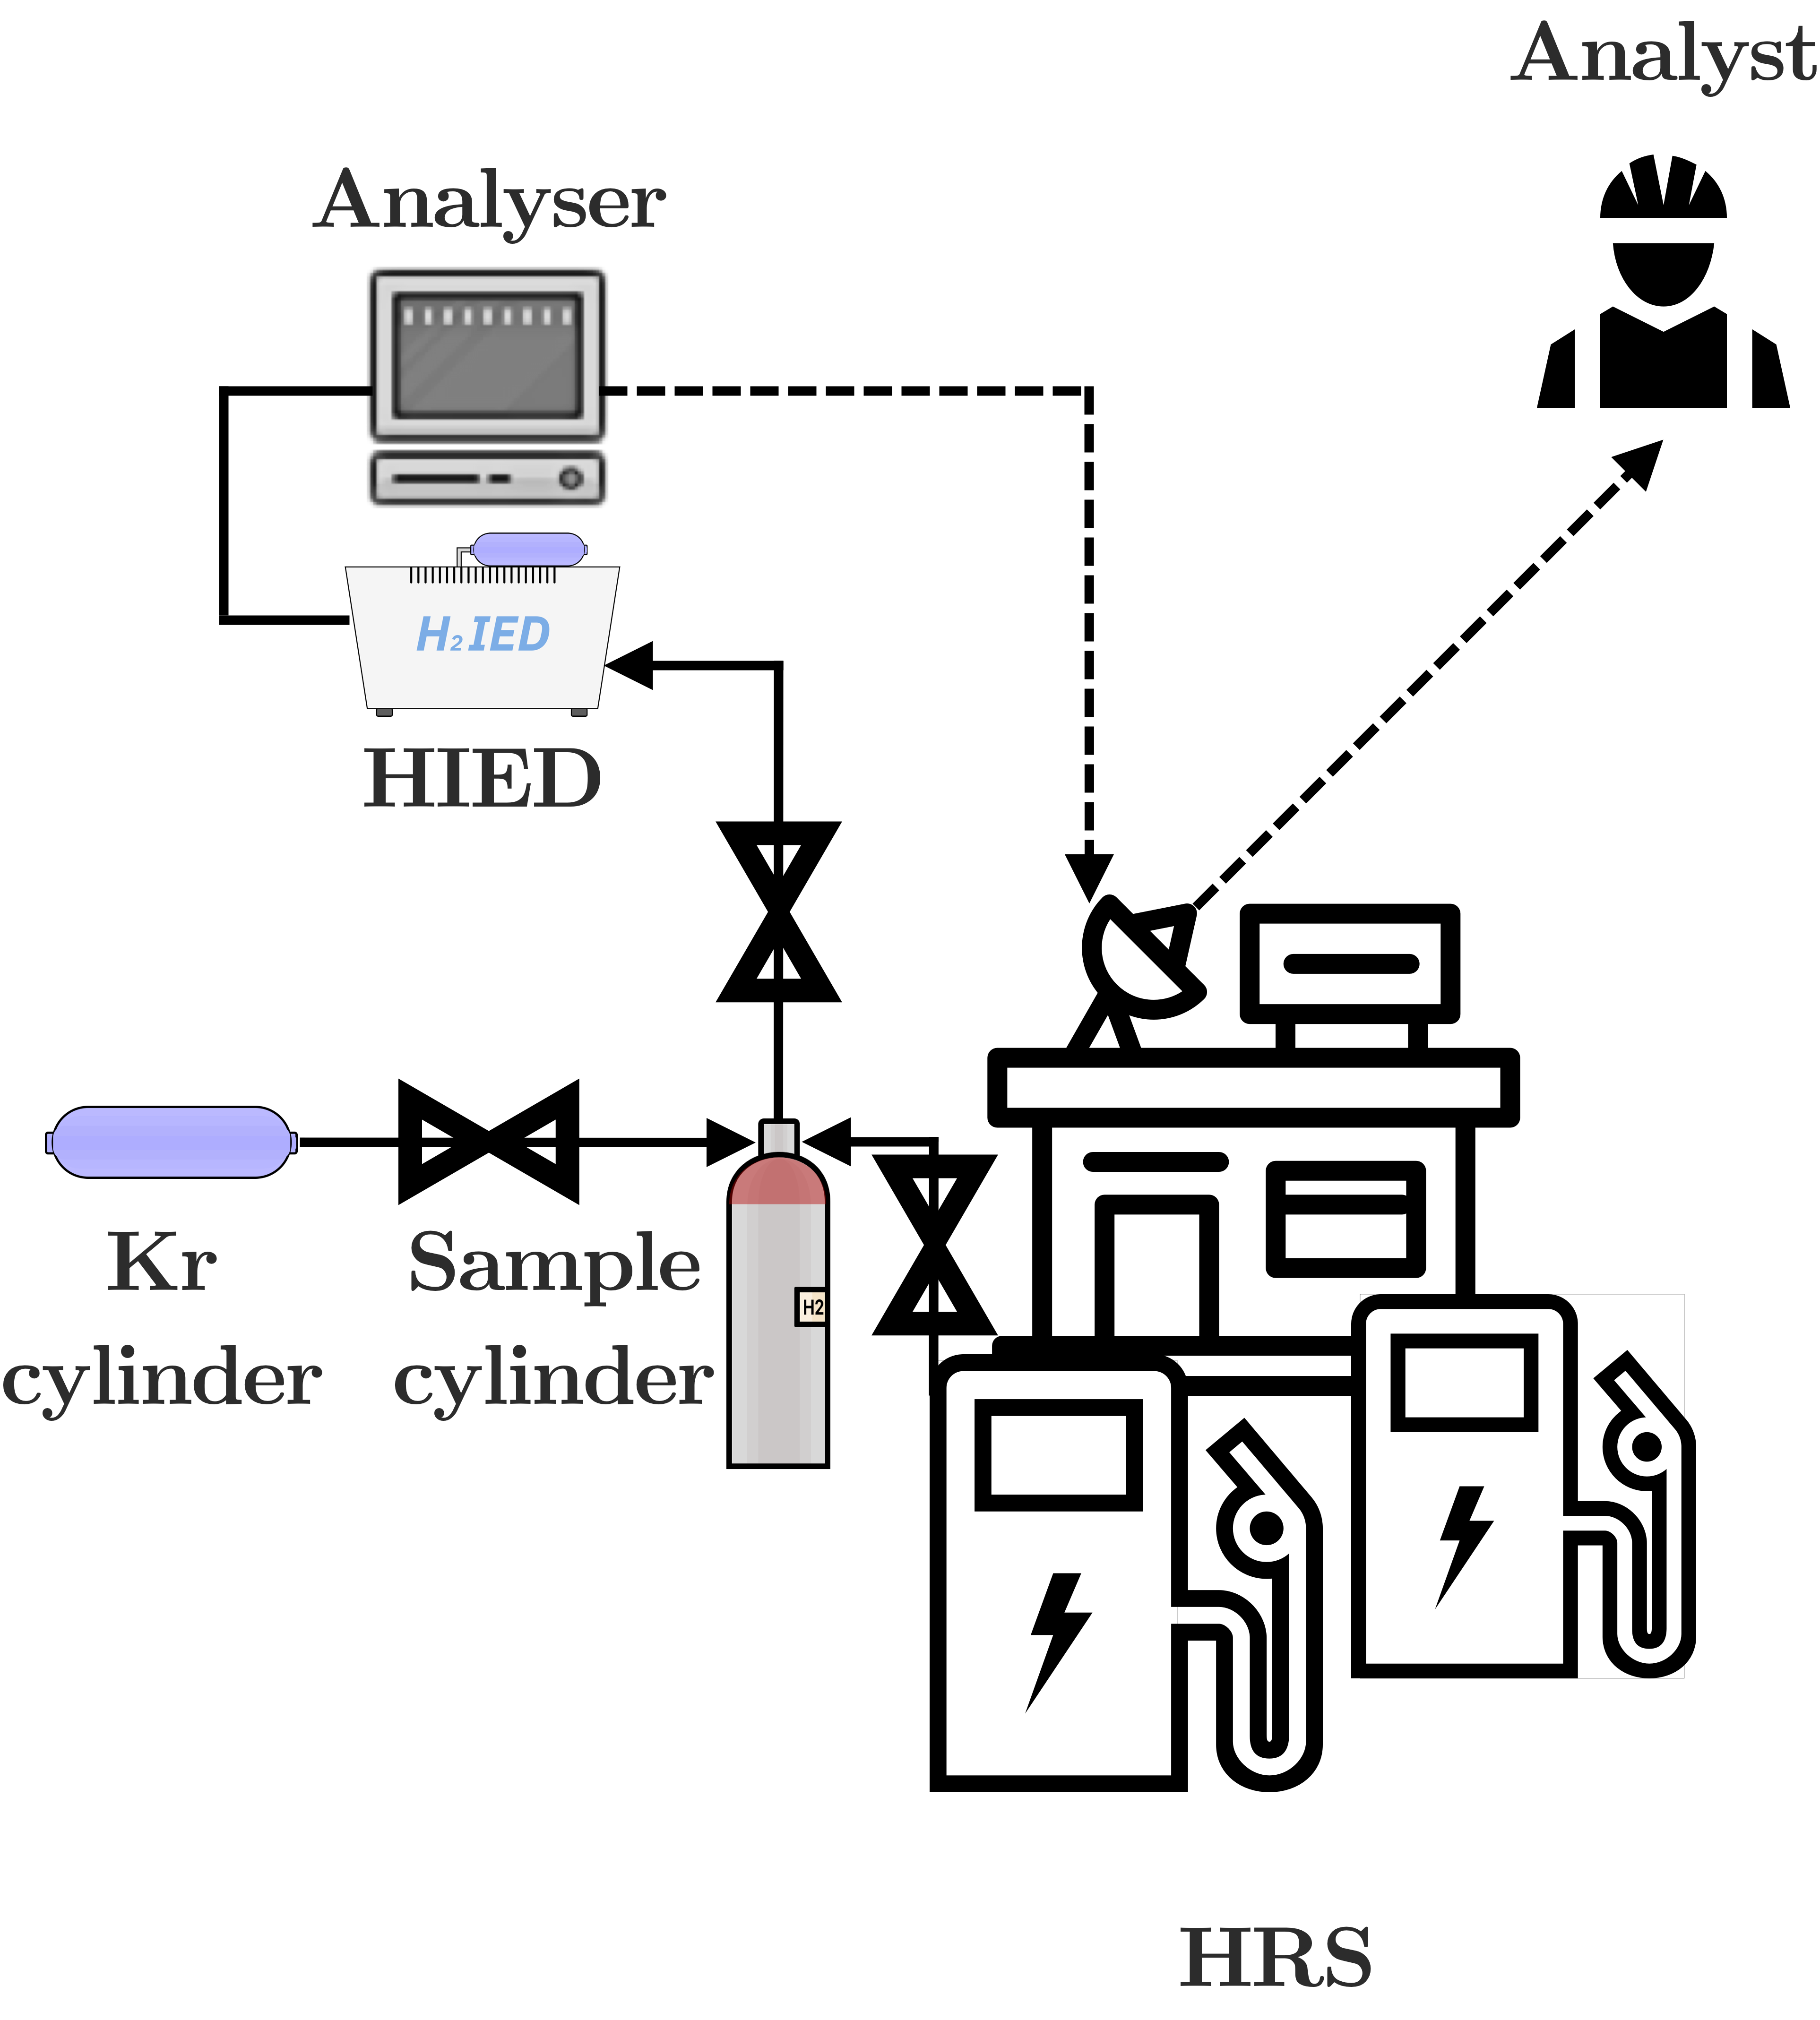
\includegraphics[width=\linewidth, keepaspectratio]{/Users/marc/Thesis/Chapter6/automation.png}
    \caption{Proposed solution for automatic quality assurance of fuel cell hydrogen at HRS's}
    \label{autoprocedure}
\end{figure}

The system could operate automatically through the use of automated valves. When a measurement is required the sample cylinder is evacuated and purged of any remaining gas, before a known mass of krypton defined in chapter 6, is spiked into the empty vessel, measured gravmetrically. The valve connecting the sample cylinder to the HRS is then opened, allowing a certain mass of hydrogen to enter the cylinder to be enriched and tested. Once enough gas has been sampled this valve can be closed, and the sample enriched. Once enrichment is complete the gas automatically passed through a dedicated analyser, tested against a standard, and the results delivered to an analyst off site. This would eliminate the costly and time consuming process of physically acquiring a sample, and transporting it to be tested, allow testing to be performed off site, and allow more flexibability for testing schedules. As the process for performing a hydrogen sample has already been defined \cite{BACQUART20205565} and could be automated with existing technology this could be the next step for impurity enrichment devices. As the market for hydrogen technology increases, modern solutions which greatly improve upon existsing processes such as these will appear increasingly viable.

NPL has recently designed a Hydrogen Purity Van, which travels to hydrogen refuelling stations and performs analysis to ISO 14687 standard on-site. Similarly to analytical labs the equipment is expensive and takes up a large amount of space due to the number of instruments required. If the HIED was integrated into the Hydrogen Purity Van then it would lower the CAPEX and make such an initiative more viable. 

One issue in the operation of the HIED is the resulting pressure of the enriched sample. Once the enriched sample has cooled the resulting pressure is normally $<$ 5 bar, which may cause some issues when performing analysis on certain instrumentation. On the flipside if the pressure is too high then the pressure relief valves will activate during the run due to the high pressure crewated during heating, throwing off the results in the same way as if a leak had formed. A solution to this would be to manufacture a membrane at a higher pressure rating in order to allow higher enrichment pressures and therefore give greater allowance for pressure drops during cooling. 

Finally it may be possible to perform in-situ measurement of some impurities within the enrichment device by incorporating chemical sensors into the enrichment vessel. Such a system would be able to automatically calculate the concentration of the impurity when it reaches the limit of detection of the sensor, combined with the non-ideal gas law enrichment factor. It would not be possible to use this type of system in conjunction with the tracer enrichment method due to there not being chemical sensors avaliable for krypton. A similar system could be created by connecting the enrichment device to a gas analyser and sampling throughtout the enrichment, for example with a GC-PDHID this could be done at 10 minute intervals. This has the advantage of being able to measure all impurities in situ, not just ones that have avaliable chemical sensors, however has the disadvantage of taking up an expensive piece of equipment for potentially days at a time. 

\subsection{Additional use cases}
There is scope for using the impurity enrichment technique for gases other than hydrogen. Dense ceramic membranes which are permaselective to oxygen are in the research stage, \cite{LIU2005103} and could potentially be inserted into the enrichment device as is to provide this analysis if needed. Another alternative could be to enrich impurities in water to provide a similar analysis. As evidence that pollutants in water are increasing at alarming levels, and are increasingly dangerous to our health, there may be increased scope for water impurity analysis in the future. \cite{marketresearchfirm}

\section{Other hydrogen impurity measurement challenges}
This thesis mainly focused on a technique which is used for off-line analysis of impurities in fuel cell hydrogen. There is still a need for on-line monitoring of impurities at HRS's as stated by ISO 19880-8:2019. In a report performed for the MetroHyve project they concluded that no such devices capable of perfoming on-line sensing exist. Some of the methods used in this thesis, in particular the use of simulations to predict the suitability of a material for a given purpose, could prove useful when researching in this area. 

\section{Closing remarks}
This thesis explored the use of a number of experimental and computational methods to find and test the best membrane for enriching hydrogen impurites to enable testing at a low cost, making the process accessable to a larger number of measurement providers. A commercialised device was designed and has been sold, able to provide purity analysis to within 2\% of the original value. An appropriate membrane composition was found although further work is required to manufacture a palladium coated ceramic hollow fibre which is able to withstand the conditions required for enrichment. DFT proved to be a useful tool in screening of allows, in particular those resistent to sulphur impurities, however further work must be done to define an appropriate model for the interaction of the alloy surfaces and carbonaceous impurities which the model was not able to accurately predict. More impurities which are not included in the ISO standard, such as siloxanes, are also worthwhile investigating due to the increasing number of sources for hydrogen production processes increasing the liklihood of new impurities coming into contact with palladium membrane systems.


\bibliographystyle{unsrtnat}
\bibliography{library.bib}